% This file was created with tikzplotlib v0.10.1.
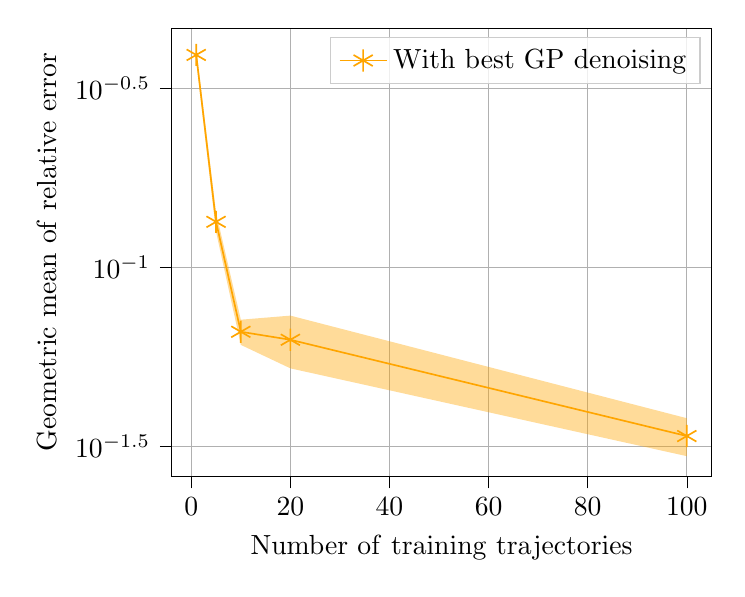
\begin{tikzpicture}

\definecolor{darkgray176}{RGB}{176,176,176}
\definecolor{lightgray204}{RGB}{204,204,204}
\definecolor{orange}{RGB}{255,165,0}

\begin{axis}[
legend cell align={left},
legend style={fill opacity=0.8, draw opacity=1, text opacity=1, draw=lightgray204},
log basis y={10},
tick align=outside,
tick pos=left,
x grid style={darkgray176},
xlabel={\(\displaystyle \mathrm{Number \ of \ training \ trajectories }\)},
xmajorgrids,
xmin=-3.95, xmax=104.95,
xtick style={color=black},
y grid style={darkgray176},
ylabel={\(\displaystyle \mathrm{Geometric \ mean \ of \ relative \ error }\)},
ymajorgrids,
ymin=0.0260468415425964, ymax=0.466377451244302,
ymode=log,
ytick style={color=black}
]
\path [fill=orange, fill opacity=0.4, semithick]
(axis cs:1,0.409056968724872)
--(axis cs:1,0.376589402124321)
--(axis cs:5,0.125902384109127)
--(axis cs:10,0.0607804138457918)
--(axis cs:20,0.0522579528563048)
--(axis cs:100,0.0296967427531365)
--(axis cs:100,0.0379157280727796)
--(axis cs:100,0.0379157280727796)
--(axis cs:20,0.073374207130092)
--(axis cs:10,0.0714742460827114)
--(axis cs:5,0.142441339175987)
--(axis cs:1,0.409056968724872)
--cycle;

\addplot [semithick, orange, mark=asterisk, mark size=4, mark options={solid}]
table {%
1 0.392823219299316
5 0.13417187333107
10 0.066127322614193
20 0.0628160759806633
100 0.0338062383234501
};
\addlegendentry{With best GP denoising}
\end{axis}

\end{tikzpicture}
